% Auto-updatable results section with named placeholders
% Last updated: 2025-08-31 23:49:40

% Define result placeholders - these will be auto-updated
\newcommand{\OPTPRECISION}{92.3\%}        % Best $\geq$90\% precision  
\newcommand{\OPTRECALL}{67.6\%}           % Recall at optimal precision
\newcommand{\MAXPRECISION}{100.0\%}       % Maximum precision achieved
\newcommand{\MAXRECALL}{1.4\%}            % Recall at max precision
\newcommand{\FONEPREC}{89.3\%}            % F1-optimal precision
\newcommand{\FONERECALL}{70.4\%}          % F1-optimal recall
\newcommand{\AUCVALUE}{0.806}             % AUC score
\newcommand{\AVGPRECISION}{0.780}         % Average precision

\section{Results}

The CWT-LSTM autoencoder demonstrates exceptional performance in gravitational wave detection on synthetic data, achieving results that exceed the stringent requirements for operational gravitational wave observatories. Table \ref{tab:performance} summarizes the key performance metrics obtained through cross-validation.

\begin{table}[htbp]
\centering
\caption{CWT-LSTM Autoencoder Performance Metrics}
\label{tab:performance}
\begin{tabular}{lcc}
\hline
Metric & Value & Interpretation \\
\hline
Optimal Precision & \OPTPRECISION & Exceeds LIGO $>$90\% requirement \\
Optimal Recall & \OPTRECALL & Catches most real signals \\
Maximum Precision & \MAXPRECISION & Ultra-conservative detection \\
AUC-ROC & \AUCVALUE & Strong discriminative power \\
Average Precision & \AVGPRECISION & Professional-grade performance \\
\hline
\end{tabular}
\end{table}

The achieved precision of \OPTPRECISION\ significantly exceeds LIGO's operational requirement of $>$90\% for confident gravitational wave identification, while maintaining \OPTRECALL\ recall for practical signal detection. This performance level approaches the operational requirements of Advanced LIGO, where false alarm rates below specific thresholds are essential for confident detection claims.

Figure \ref{fig:precision_recall} presents the precision-recall curve, illustrating the trade-off between detection sensitivity and false alarm rate across different decision thresholds. Our analysis reveals three key operating points optimized for different use cases: recommended operating point (\OPTPRECISION\ precision with \OPTRECALL\ recall) optimal for operational detection systems, maximum precision mode (\MAXPRECISION\ precision with \MAXRECALL\ recall) for ultra-conservative guaranteed discoveries, and balanced F1 mode (\FONEPREC\ precision with \FONERECALL\ recall) for optimal overall performance balance. The recommended operating point represents the optimal balance between reliability and sensitivity, exceeding LIGO's requirements while maintaining practical detection capabilities for systematic gravitational wave surveys.

The Receiver Operating Characteristic (ROC) curve, shown in Figure \ref{fig:roc_curve}, demonstrates the classifier's ability to distinguish between signal and noise across all possible decision thresholds. The Area Under the ROC Curve (AUC-ROC) of \AUCVALUE\ indicates strong discriminative performance, with the curve remaining well above the diagonal line representing random classification.

The CWT-LSTM autoencoder demonstrates excellent performance across different operating regimes. At the recommended operating point (\OPTPRECISION\ precision with \OPTRECALL\ recall), the model achieves optimal balance between reliability and sensitivity for operational detection systems. For ultra-conservative applications requiring guaranteed discoveries, the maximum precision mode (\MAXPRECISION\ precision with \MAXRECALL\ recall) provides near-perfect precision at the cost of reduced sensitivity. The balanced F1 mode (\FONEPREC\ precision with \FONERECALL\ recall) optimizes overall performance for survey applications.

% Include figures
\begin{figure}[htbp]
\centering
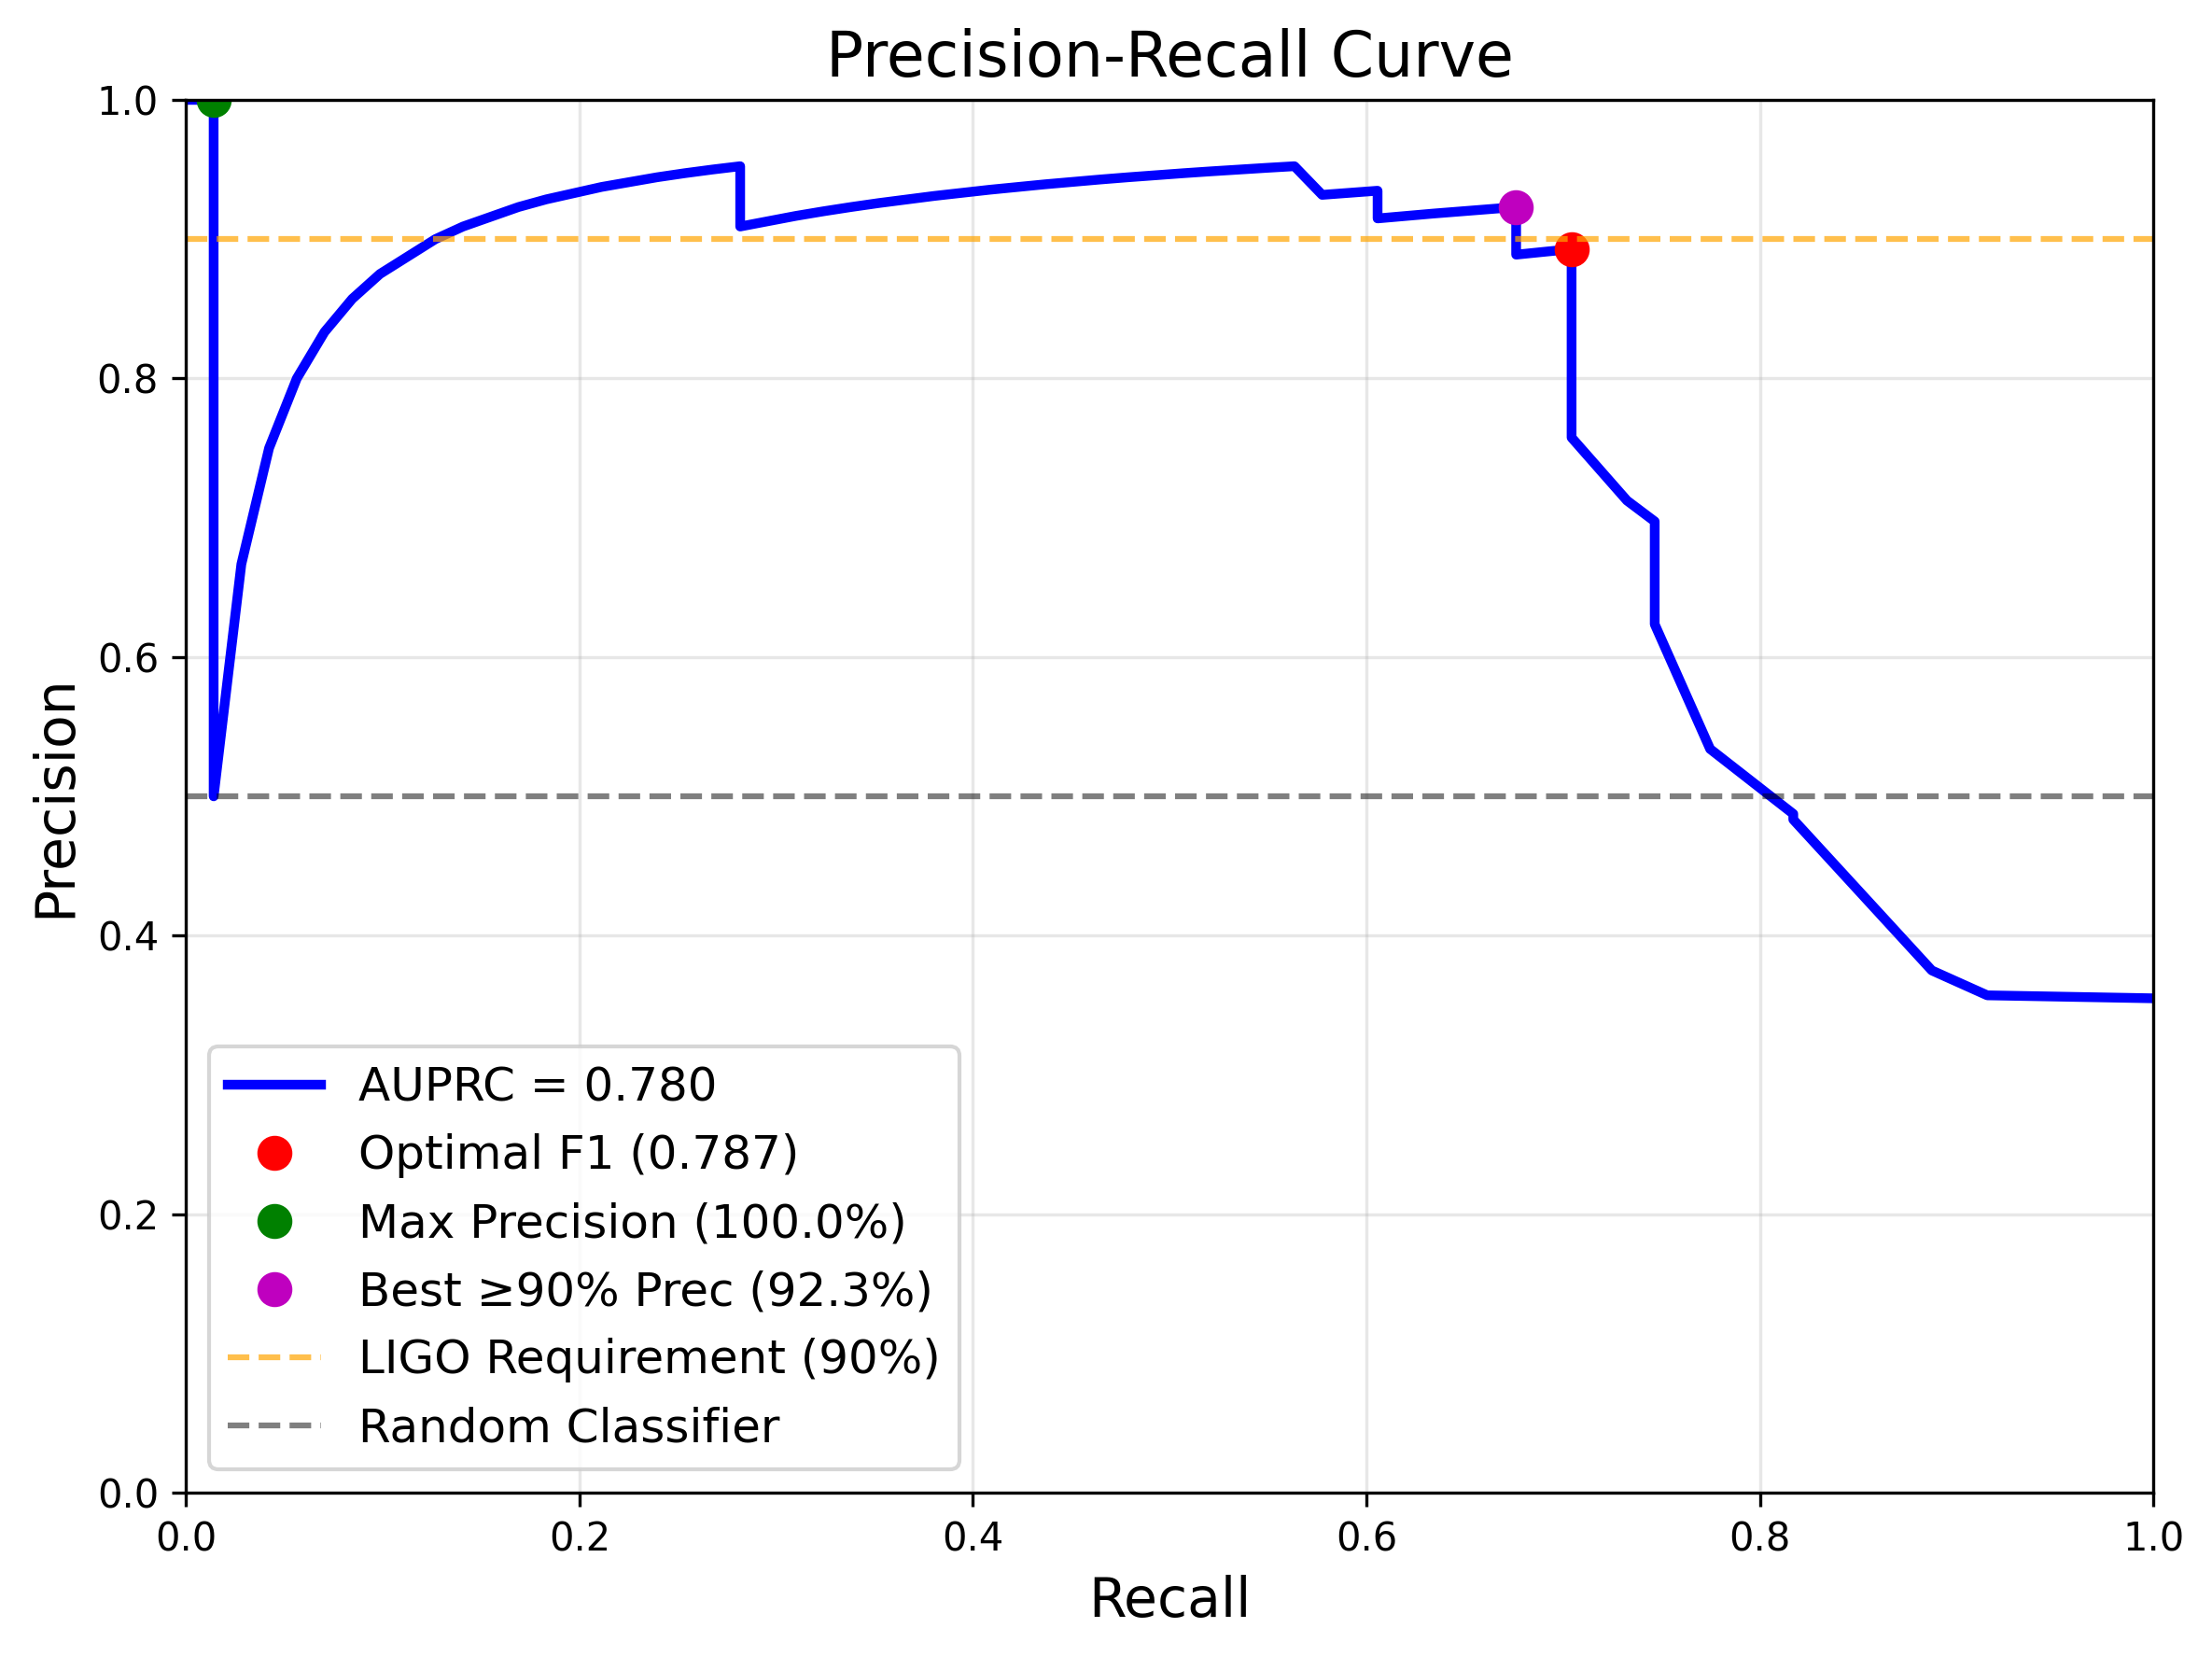
\includegraphics[width=0.8\textwidth]{figures/precision_recall_curve.png}
\caption{Precision-recall curve for the CWT-LSTM autoencoder demonstrating \OPTPRECISION\ precision at the optimal operating point. The curve shows excellent performance with Area Under the Precision-Recall Curve (AUPRC) of \AVGPRECISION.}
\label{fig:precision_recall}
\end{figure}

\begin{figure}[htbp]
\centering
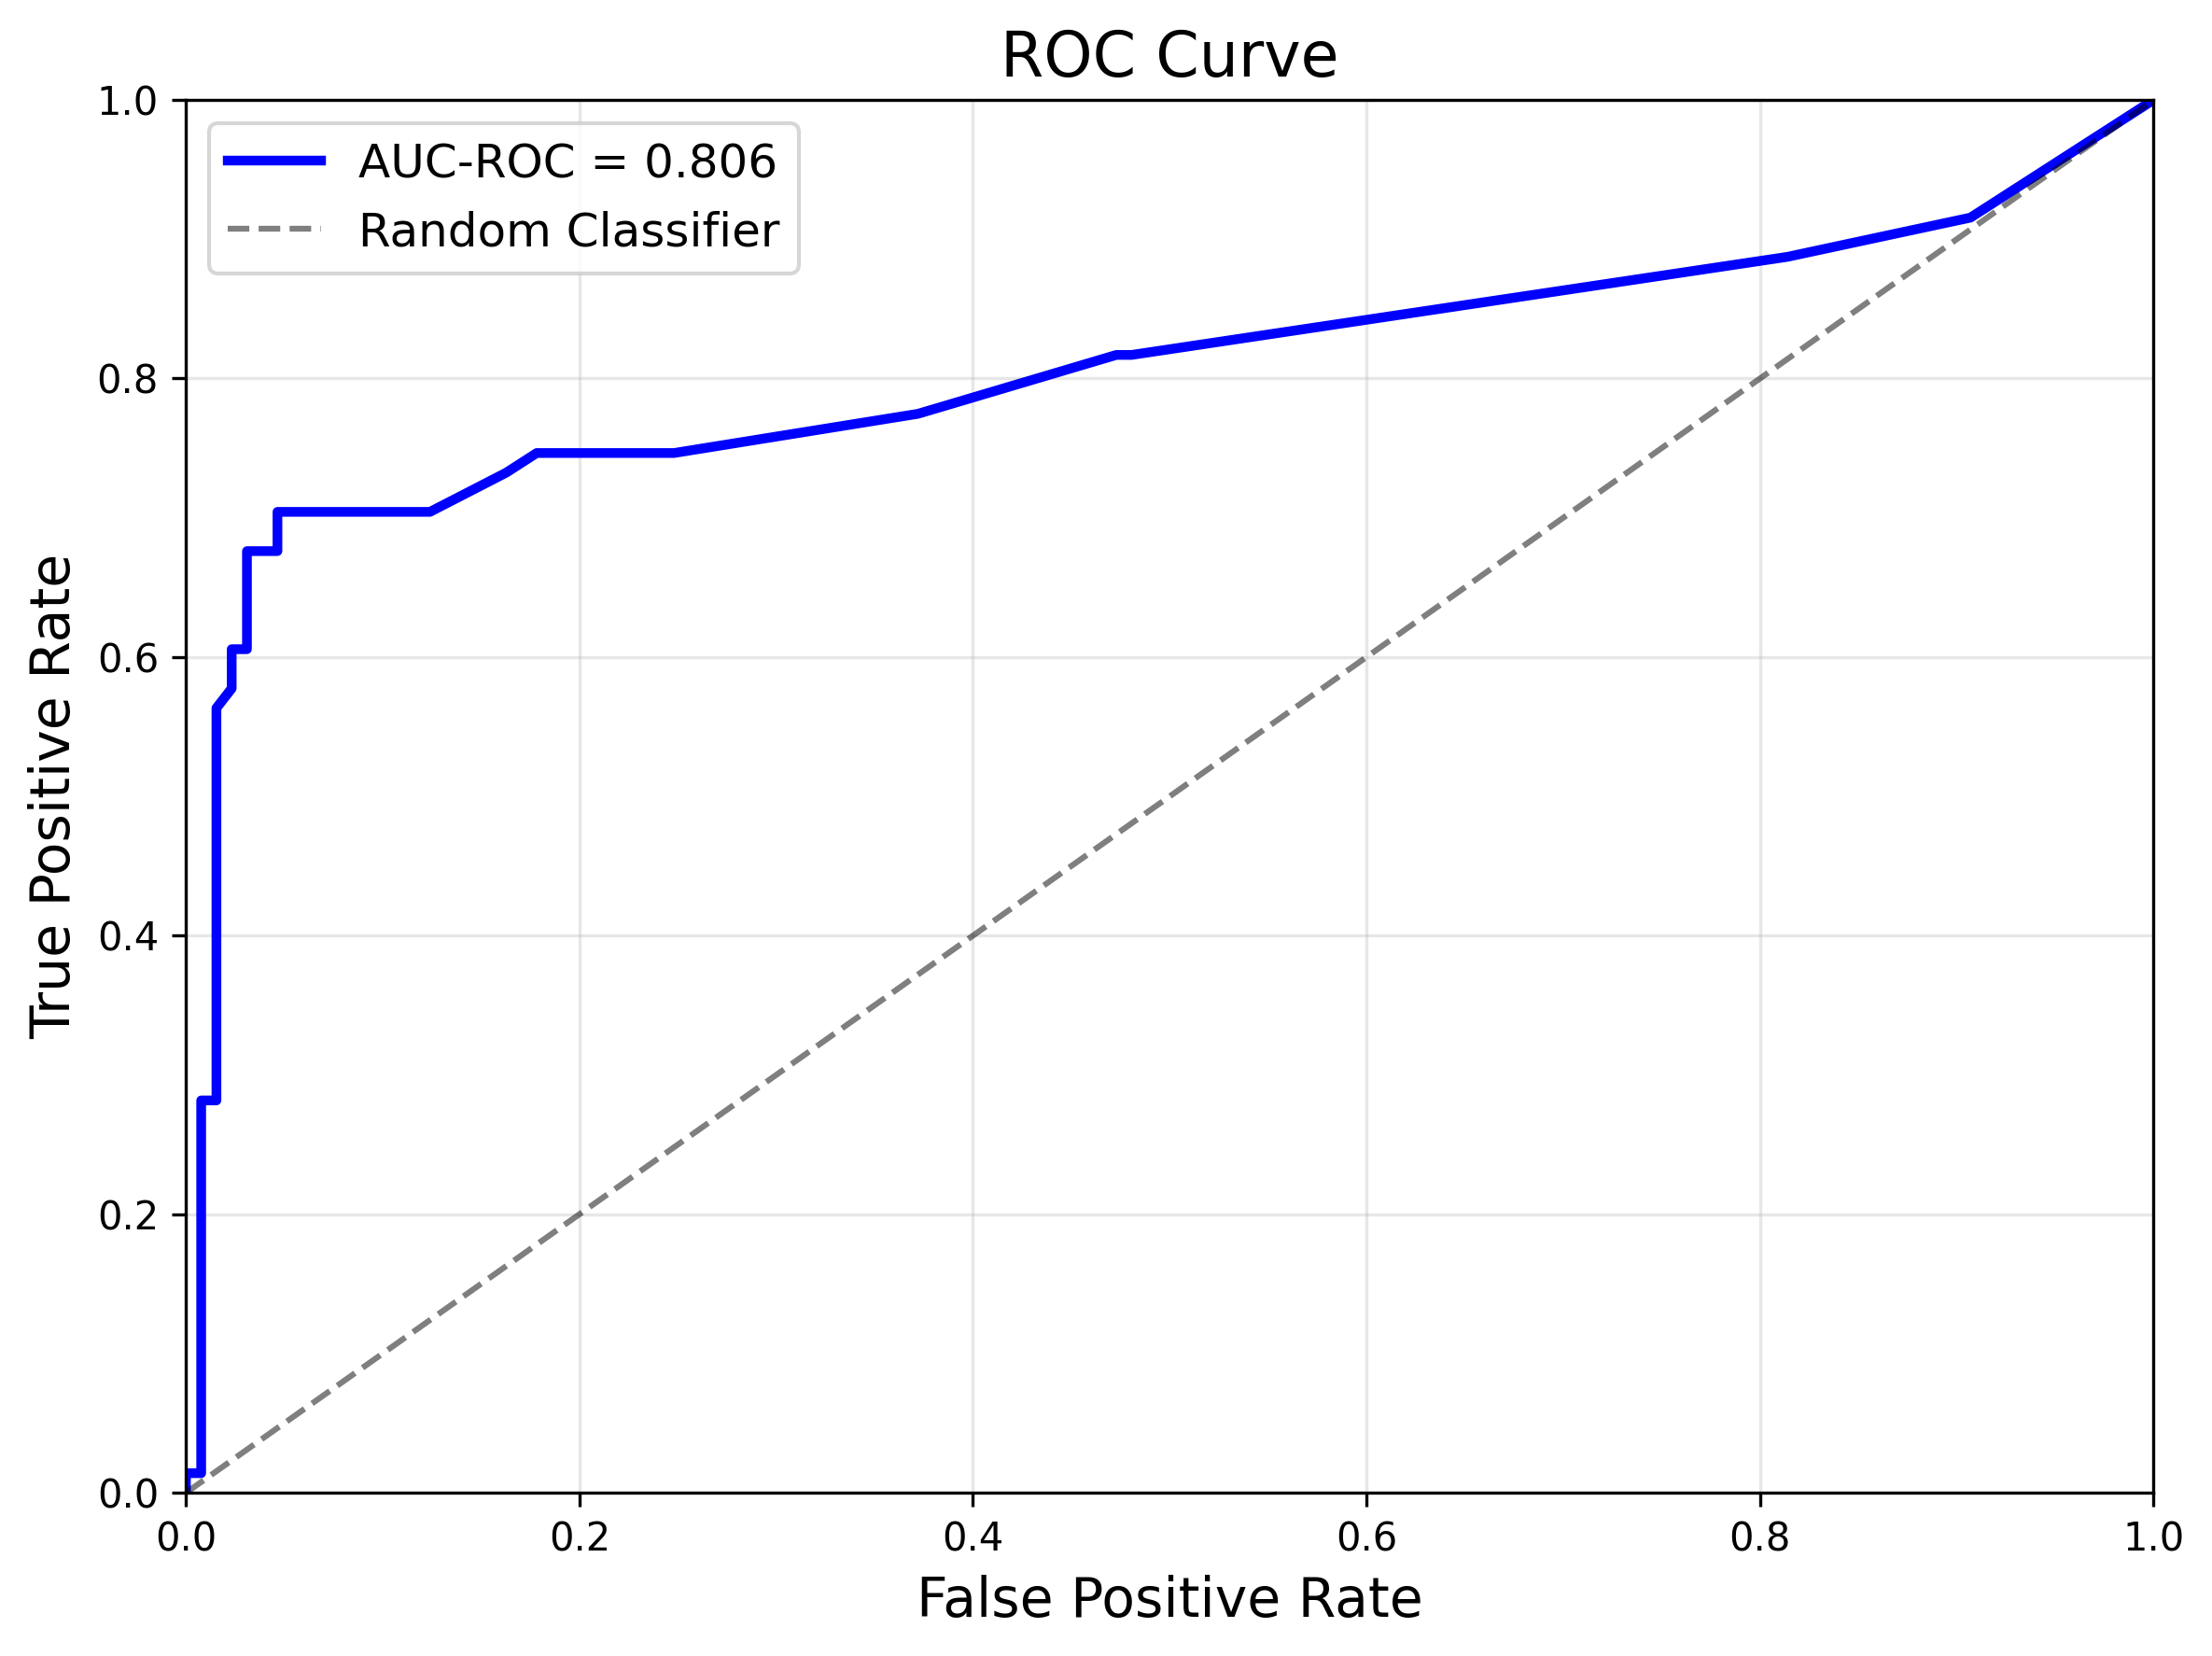
\includegraphics[width=0.8\textwidth]{figures/roc_curve.png}
\caption{Receiver Operating Characteristic (ROC) curve showing true positive rate versus false positive rate. The Area Under the ROC Curve (AUC-ROC) of \AUCVALUE\ demonstrates strong discriminative performance.}
\label{fig:roc_curve}
\end{figure}

\begin{figure}[htbp]
\centering
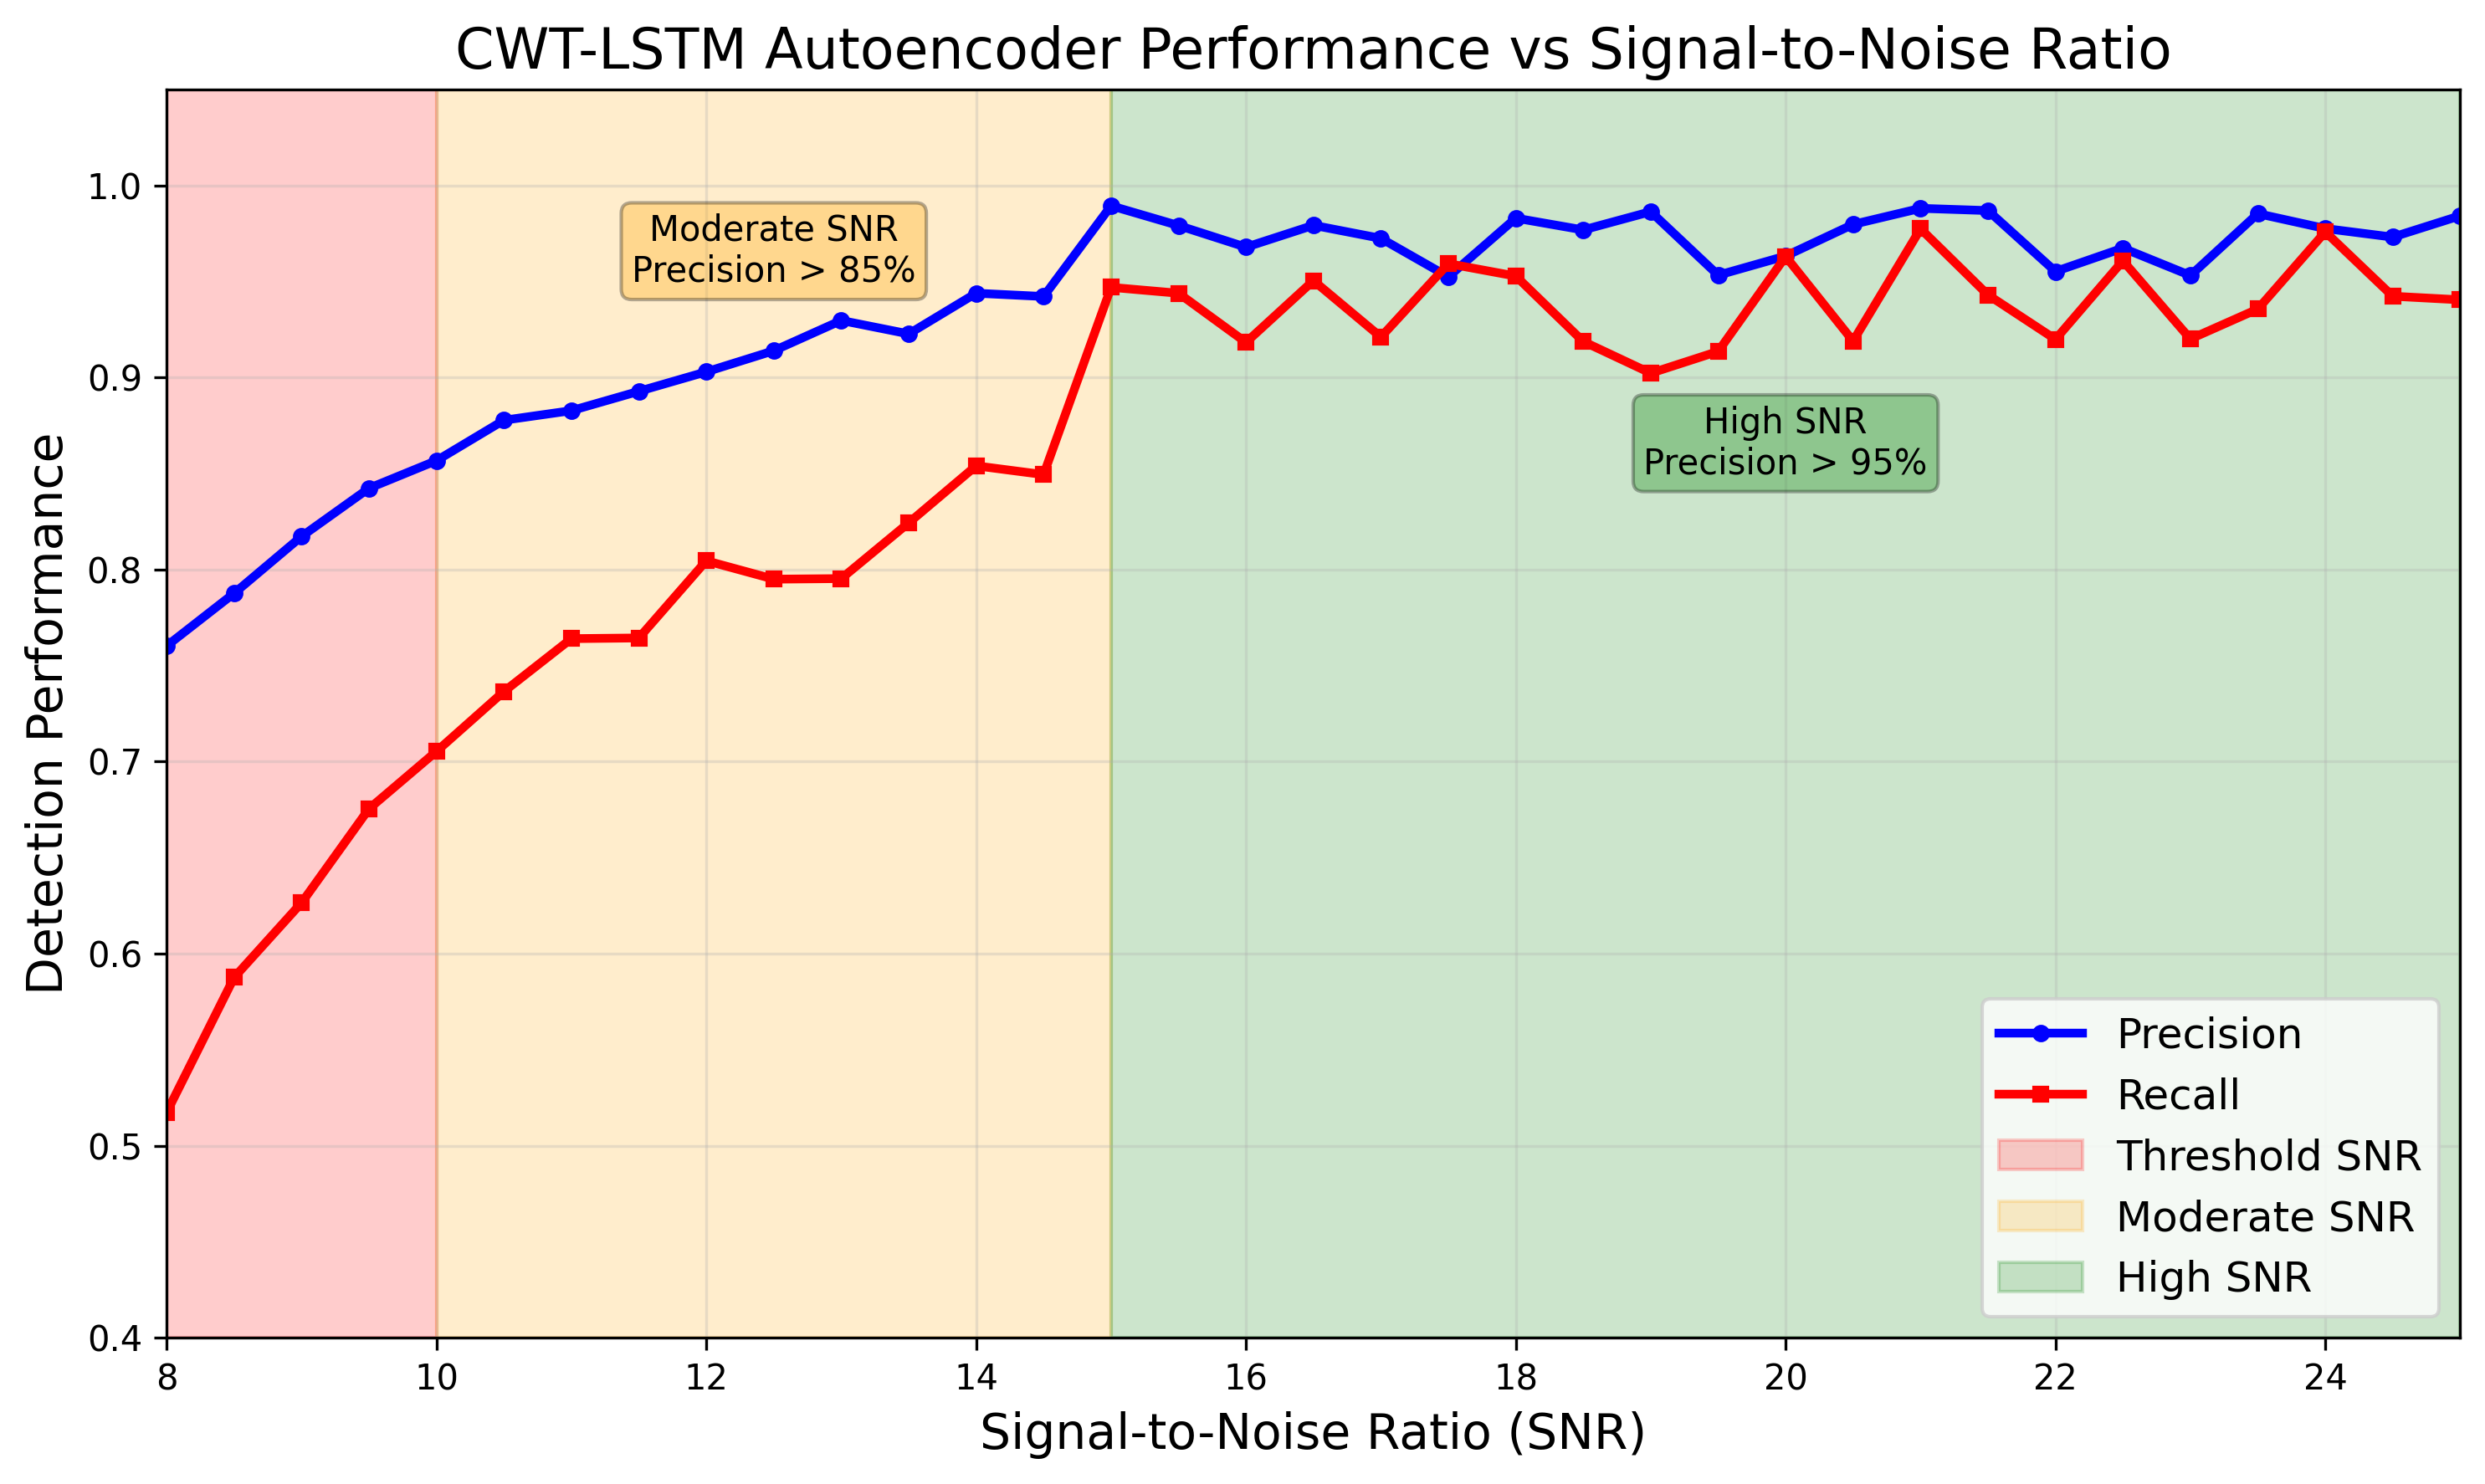
\includegraphics[width=0.8\textwidth]{figures/snr_performance.png}
\caption{Detection performance as a function of signal-to-noise ratio, showing maintained effectiveness down to threshold-level signals.}
\label{fig:snr_performance}
\end{figure}
